\documentclass[a4paper]{article}
\usepackage[english]{babel}
\usepackage{amsmath}
\usepackage{graphicx}
\usepackage[justification=centering]{subcaption}
\usepackage{placeins}
\usepackage{booktabs}
\usepackage{tikz}
\usepackage{textcomp}

\title{Building Evacuation}
\author{Maarten de Jonge \\
        Edwin Odijk \\
        Roelof van der Heijden}

\begin{document}

\maketitle

\section{Introduction}
In this report we simulate people escaping from a burning building using the BDI framework in NetLogo. We create an environment with people and fire randomly distributed throughout the building. People randomly walk through the building until they spot fire, at which point they try to run towards the escape and alarm any others they meet along their way. The simulation ends when all people either escaped or died in a fire.

Using this simulation, we aim to find what affects the speed and survival rate of such an evacuation.

Additionally, we describe the NetLogo implementation, explaining the functions of buttons and how they are implemented.

\section{Simulation implementation}
\FloatBarrier
The simulation environment is a \(60\times 40\) grid, representing an office space (Figure~
\ref{fig:sp}). The walls (black tiles) were hand-drawn to craft a somewhat
realistic layout of rooms and hallways. In this case, we chose to base the layout on floor 1 of the B building of Amsterdam Science Park. One exit (green tile) is placed
at a preset position, accompanied by a variable number of randomly placed initial fires (red tiles). 
%Care is taken to ensure the exit is reachable, i.e. it is not inside a wall or on fire.

\begin{figure}[h!]
  \centering
  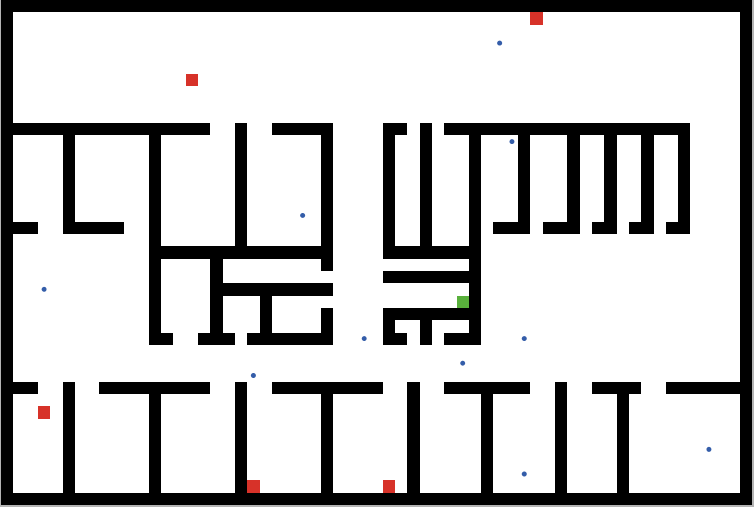
\includegraphics[width=0.7\textwidth]{sp.png}
  \caption{Science Park building B floor 1, with random fires (red) and preset exit (green) at \(t=0\).}
  \label{fig:sp}
\end{figure}

A variable amount of people (ranging from 1 to 25) is spawned, again making sure not to place them inside walls or fires. 

\subsection{Agents}
The agents represent people trying to escape the burning building.
Following the BDI framework, the agents possess the beliefs, desires and
intentions described in Table~\ref{tbl:bdi}.
\begin{table}[h!]
  \centering
  \begin{tabular}{lll}
    \toprule
    Beliefs & Desires & Intentions \\
    \midrule
    Locations of walls & Roam & Roam around \\
    Locations of fire & Escape & Panicked \\
    Location of exit &  & Move towards exit \\
    & & Alarm other agents of fire \\
    \bottomrule
  \end{tabular}
  \caption{Agents in the BDI framework}
  \label{tbl:bdi}
\end{table}

Additionally, each agent has a variable vision radius for detecting fires 
and a radius for detecting people to alarm.

Next we will discuss the agents beliefs, desires and intentions more in depth. A visual overview on how the agent changes its desires and intentions can be seen in Figure~\ref{tikz:flow}.


\subsubsection{Agent Beliefs}
There are three concepts that comprise an agents belief state: the location of walls, location of fire and the location of the exit. Both the location of the walls and  the location of the exits are assumed to be known by the agent at the start of the simulation. The reasoning behind this is that we assume the agent to have become sufficiently familiar with the building before a fire has broken out. 

On the other hand, an agent is not aware of the locations of any fires at the start of the simulation. When the agent encounters any fires during the simulation as part of his movement, he will add these locations to his own belief state. When the agent tries to move towards the exit, he will use the information in his belief state to try to plan a route avoiding any fire locations that he knows about. 

\subsubsection{Agent Desires}
We have chosen for a simple model of the desires of the agent: they either want to roam or escape. Initially, we set the intention of the agent to roam. As soon as the agent has become aware of any fire locations, the desire of the agent changes to escape. This means he will now try to move towards the exit, alarm other agents by sharing his beliefs on the locations of fires or be panicked. These intentions are explained below.

\subsubsection{Agent Intentions}
There are four possible intentions an agent can have. These are either \textit{roam around}, \textit{panicked}, \textit{move towards exit} or \textit{alarm other}. 

When the desire of the agent is to roam, his intention will be to roam around. This is implemented as a random movement, moving straight ahead with a high probability or otherwise turning left or right (with equal probability). This behaviour is meant to mimic normal human behaviour. We are aware that in most situations, a person would be more likely to stay put or go to a specific location, however to keep the simulation somewhat simple, we decided on this implementation.

When the desire of the agent is to escape, his intention becomes slightly more complex. If there are any other agents within vision radius, he will not move but instead share his knowledge on the locations of fires with them. This way other agents become aware of the fires as well, meaning they will move towards the exit as well. Because these agents will have a high probability to move towards the exit, they will likely share a very similar path. This means that most of the time the agents will be close towards each other and therefore within their communication range. The result would normally be that they would not move whatsoever but instead try to alarm each other continuously. 

To prevent this obviously undesired behaviour, we have hardcoded into the system to only alarm others when you have not done so in the previous tick. Otherwise, the agent will move towards the exit, ignoring the cries of the dying.

However, in doing so we inadvertently have introduced some other undesired aspect into the simulation: agents travelling in groups will now move at half speed compared to agents that move on their own towards the exit. For this reason, we have the agents alternate between the move towards exit and the panicked intentions. When an agent is panicked, it does not move, thereby effectively halving its overall speed and matching his speed with other agents moving in groups.

\subsubsection{Pathplanning}
To find their way among the complex environment of walls, people and fires,
agents make use of a simple $A^*$ search algorithm. The
heuristic function is the Manhattan distance, mimicking the way the agents
actually move. Tiles containing a wall or fire are considered inaccessible
by the algorithm, while tiles containing agents are not (as other nearby
agents are most likely also moving towards the exit, it makes no sense to plan
a detour just because someone who is moving in the same direction is blocking a
doorway).

One problem that pops up is that each agent will explore the entire
search space if the exit is blocked, taking up a lot of processing power and
slowing the simulation to a crawl. This is alleviated by assuming that because
each obstacle is permanent (fires will never go out, and walls aren't going
anywhere unless they're replaced by fire), there is no reason to keep trying
after the path calculation has failed once for an agent. As a result, these
agents will stand around waiting for their impending doom, freeing up CPU time
for their colleagues that still have a chance of making it out alive.

Another thing to note is that the planning algorithm has no preference to stay away from fires. If an agent has to move 10 steps down and 10 steps left to get to the exit, the planning algorithm will not favor going down first and left next or the other way around, even though one route may be much closer or even adjacent to tiles that are on fire. As a consequence, sometimes agents will die as the fire spreads to a new tile while this could have avoided easily had the agent chosen another path to the exit.

\begin{figure}[!ht]
  \centering

\captionsetup{justification=centering,margin=1cm}
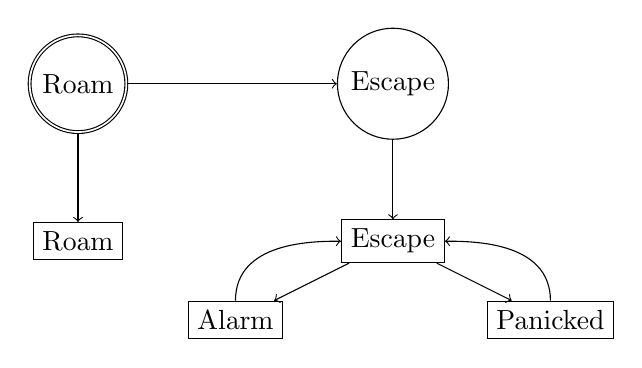
\begin{tikzpicture}
\path 
(2,0) node[circle, double, draw] (des-roam) {Roam}
(6,0) node[circle, draw] (des-escape) {Escape}
(2,-2) node[draw] (roam) {Roam}
(6,-2) node[draw] (escape) {Escape}
(4,-3) node[draw] (alarm) {Alarm}
(8,-3) node[draw] (panic) {Panicked};

%\draw[->] (init) -- node {} (des-roam);
\draw[->] (des-roam) -- node {} (des-escape);
\draw[->] (des-roam) -- node {} (roam);
\draw[->] (des-escape) -- node[above,sloped] {} (escape);
\draw[->] (escape) -- node[above,sloped] {} (alarm);
\draw[->] (alarm) .. controls +(up:1cm) and +(left:1cm) .. node[above,sloped] {} (escape);
\draw[->] (escape) -- node[above,sloped] {} (panic);
\draw[->] (panic) .. controls +(up:1cm) and +(right:1cm) .. node[above,sloped] {} (escape);
%\draw[->] (init) -| node[near start,below] {label} (roam);
\end{tikzpicture}
\caption{Flowchart of agent desires and intentions. Desires are encircled, and intentions are in rectangles. Roam is the initial desire.}
\label{tikz:flow}
\end{figure}


\subsection{NetLogo Controls}
To give more insight in the workings of this simulation, we provide a overview below of the controls implemented in NetLogo, as not all of them may be self-explanatory.

\subsubsection{Draw, Save and Clear walls}
Walls used by the simulation are hand drawn and saved in a separate txt file. Upon running \texttt{Setup}, the file is read to redraw the walls.

To use the function, first ensure that \texttt{Setup} has been run at least once. If walls are already present, you can click \texttt{clear\_walls} (thereby removing the txt file) and run \texttt{Setup} again to redraw the environment with an empty sheet. Clicking \texttt{draw\_walls} allows you to start drawing with the environment. When you are finished, click \texttt{draw\_walls} again to stop drawing, then click \texttt{save\_walls} to save the new environment, which will now be redrawn every time \texttt{Setup} is run.

\subsubsection{Throttle Speed}
As the simulation may slow down at times, it may be preferable to watch the simulation at a constant speed. Turning \texttt{throttle\_speed} on slows all steps to an equal speed of 100 milliseconds. This does mean that the overall speed of the simulation is slowed down, however, so this should be off when swift simulations are desired.

\subsubsection{Fire Spread Rate}
Controls the speed at which fire spreads. At every step, for every red tile's neighbours, they are set on fire with a certain probability defined by \texttt{fire\_spread\_rate} per mille. As a consequence, tiles that are not on fire but are adjacent to two or more tiles that are have a higher probability to be set on fire.

\subsubsection{Vision}
The properties \texttt{fire\_vision} and \texttt{person\_vision} control the vision in which each agent can observe nearby fire or other agents respectively. This vision is represented by an invisible circle around the agent, with a radius equal to the value defined on the slider. We do not take into accounts any walls between the agent and the fire or the other agents.

\FloatBarrier
\section{Experiments}
For this experiment, we investigate the effect of the number of people on the overall survival rate. To do so, we set up a basic case with the following properties:
\begin{itemize}
\item Number of starting fires: 1
\item Rate at which fire spreads: 20\textperthousand
\item Agent FoV for spotting fires: 3
\item Agent FoV for spotting other agents: 4
\item Addition or removal of walls: 4
\end{itemize}

We then vary the number of people between 5, 10 and increments of 10 onwards to 100. In total, these are 11 separate experiments.

To analyze the overall survival rate, we track for each agent when it escapes or dies. This is measured in the number of ticks since the simulation started. For each experiment, we run the simulation 16 times and average the results for each timestep (ticks). This results in two graphs, one for the number of deaths over time and one for the number of escapees over time.

We expect that, as the number of persons increase, the variance in the survival rate will increase as well. However, when the number of persons gets sufficiently large, when someone spots a fire it might be communicated effectively throughout the population, thereby increasing the survival rate and decreasing the variance. We can easily calculate an upper bound for this to occur. 

The environment is \(60\times 40\), but the outside is walls. So the effective area is \(59 \times 39 = 2301\) tiles. The default communication vision for agents is 4. For ease of calculation, we shall fit a square of area 8 inside this circle. If all the agents are evenly spaced, then we need 288 agents to monitor the entire simulation.

In practice, it is likely that we shall witness this effect already with a far smaller number of agents, as the calculation above disregards (among other things) the movement of agents. Exactly how many, we will try to find out with our experiments.

%\begin{itemize}
%\item Can we prevent traffic jam behaviour?
%\item How much do the following properties affect overall survival rate?
%\begin{itemize}
%\item Rate at which fire spreads
%\item Whether agents have prior knowledge of exit locations
%\item The ratio between agents that prioritize saving themselves over saving others
%\end{itemize}
%\end{itemize}

\section{Results}
The results of our experiments can be seen in Figure~\ref{fig:escape}. Here we can see that the percentage of survivors is the highest for 100 agents, the highest value that we tested. Second is 90 agents, then 80 and this trend more or less continues for smaller number of agents. We have also run 2 tests with 200 agents, both having an escape rate of around 90\%. This indicates that our hypothesis, that a bigger number of agents results in more survivors, holds true. 

\begin{figure}[ht]
  \centering
  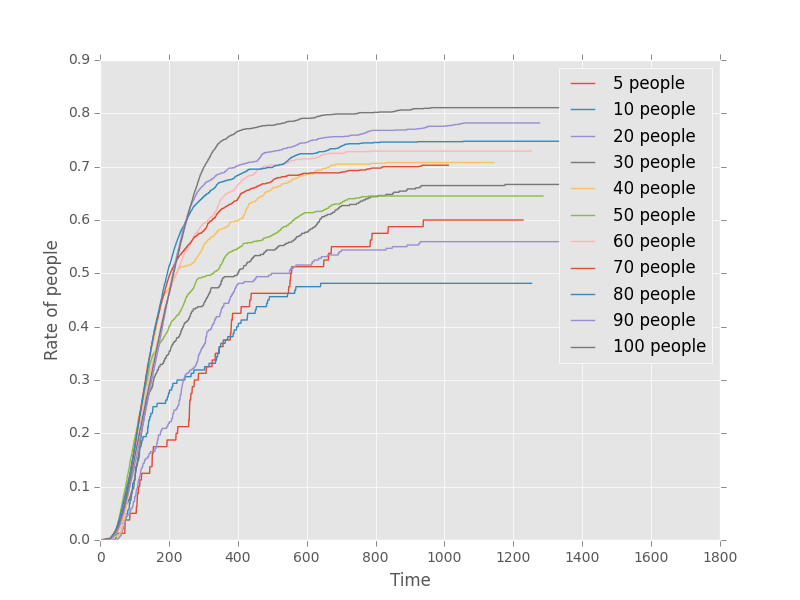
\includegraphics[width=\linewidth]{escaperate.png}
  \caption{Percentage of escapees.}
  \label{fig:escape}
\end{figure}

With data extracted from the same set of simulations, we have created Figure~\ref{fig:deaths}. This figure pictures the number of deaths over time. As is to be expected, we see that the higher the number of agents, the smaller the percentage of deaths is. 

\begin{figure}[ht]
  \centering
  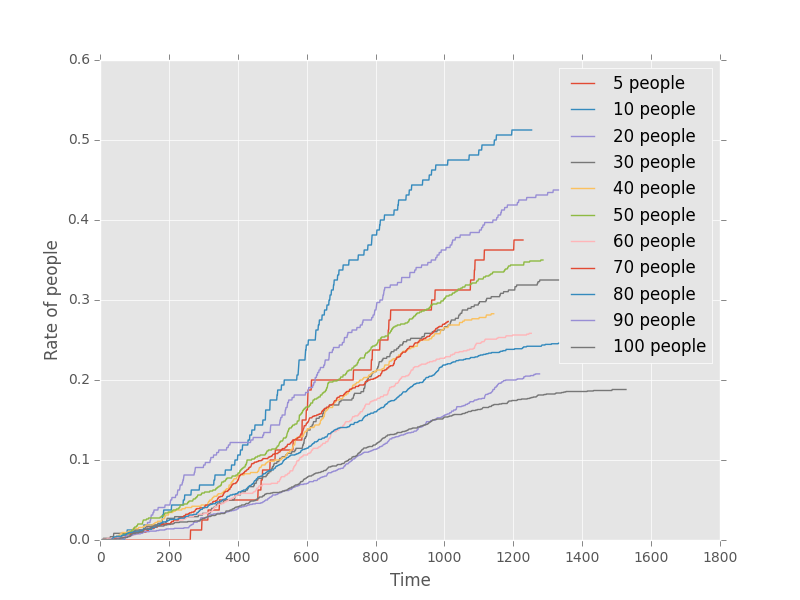
\includegraphics[width=\linewidth]{deathrate.png}
  \caption{Percentage of victims.}
  \label{fig:deaths}
\end{figure}

Another interesting behaviour we have found is that especially for simulations with many agents, a long queue is formed heading for the exit. Because of the communication protocol, an agent only moves every other tick. To be more precise, it moves when there is a free spot to move to. The pathfinding does not try to find alternative routes towards the exit if the current route is blocked by agents. Therefore, a long line of maybe 40--60 agents is formed towards the exit, while in the meantime a fire is growing literally 1 tile away from the last person in line. A more intelligent agent would take a longer route towards the exit, if it exists, just to be farther away from the fire. Our agents are incapable of this more advanced behaviour, resulting in (unnecessary) casualties. 

\section{Conclusion}
For this project we have built a simple building evacuation simulation in NetLogo. The agents in this simulation can detect fire, navigate towards a known exit and alarm others of the fire on their way. We have ran multiple simulations with varying number of agents, to examine the survival in these cases. We hypothesised that the more agents are in the simulation, the higher the survival rate would be, due to earlier detection of the fire and the faster alarming of others. We have found from the data evidence that supports our hypothesis. 

\section{Future Work}
There are various potential improvements to the simulation. One easy extension would be to incorporate ``Fire detector'' agents. These agents would have a higher fire vision and communication radius than other agents, but would be stationary and not die in fire. This would probably increase the survival rate if the fire detectors are space evenly in the environment.

Regarding the simulation environment, it
would be interesting to automatically generate an office layout based on some
parameters (e.g. number of exits, wall density, width of corridors, number of
open areas). This would allow for research to be done into the effect of the
layout on, for instance, the survival rate or some measure of traffic congestion.

The agents themselves could be parameterised by some measure of personality; for
example, they could have a probabilistic bias towards warning their colleagues,
or conversely a bias towards saving themselves without regards for the others.
This could even be extended to replicate real-world fire safety procedures where
certain agents (presumably wearing fluorescent yellow jackets) are tasked with
making sure all the other agents are aware of the fire before fleeing themselves.

Lastly, improvements could be made to the communication protocol. For example, an agent could track the minimum knowledge other agents have about fires. That way he would be able to figure out when alarming someone would be useless, as the agent already is aware of the fact that the other agent knows at least as much as himself.

\end{document}
